\documentclass[11pt]{article}

\usepackage{xcolor}
\usepackage[T1]{fontenc}
\usepackage{tabularx}
\usepackage{palatino}
\usepackage{courier}
\usepackage{alltt}
\usepackage{longtable}
\usepackage[french]{babel}
\usepackage[utf8]{inputenc}
\usepackage{float} 
\usepackage{url} 
\usepackage{ocamldoc}
\usepackage{algpseudocode}
\usepackage{algorithm}
\usepackage{amsmath,amssymb,graphicx,enumerate,calc,ifthen}


\DeclareTextSymbol{\QT}{T1}{39}
\DeclareTextSymbol{\COMMA}{T1}{44}
\DeclareTextSymbol{\COLON}{T1}{58}
\DeclareTextSymbol{\SC}{T1}{59}
\DeclareTextSymbol{\BS}{T1}{92}
\DeclareTextSymbol{\CI}{T1}{94}
\DeclareTextSymbol{\TI}{T1}{126}
\definecolor{navy}{rgb}{0.15, 0.15, 0.45} 
\definecolor{myblue}{rgb}{0.25, 0.25, 0.645} 
\definecolor{darkred}{rgb}{0.845, 0.125, 0.125} 
\definecolor{grey}{rgb}{0.4, 0.4, 0.4} 
\definecolor{darkgreen}{rgb}{0.125, 0.845, 0.125} 
\definecolor{leaf}{rgb}{0.1, 0.9, 0.1} 

\newcommand{\mlkeywordA}[1]{\mbox{\color{cyan}{\textbf{\texttt{#1}}}}}
\newcommand{\mlkeywordB}[1]{\mbox{\color{navy}{\textbf{\texttt{#1}}}}}
\newcommand{\mlkeyword}[1]{\mbox{\color{red}{#1}}}
\newcommand{\mloperator}[1]{\mbox{\color{darkgreen}{#1}}}
\newcommand{\mlmodulename}[1]{\mbox{\color{navy}{#1}}}
\newcommand{\mlstring}[1]{\mbox{\color{navy}{#1}}}
\newcommand{\mlcomments}[1]{\mbox{\color{grey}{#1}}}
\newcommand{\mlcodeline}[2]{\tiny\sl #1 & \begin{minipage}[c]{0.8\linewidth}\begin{alltt}\mbox{#2}\end{alltt}\end{minipage}\\}
% ---------------------------------------------------------------------

%\floatstyle{boxed} 
\restylefloat{figure}

%%%%%%%%%% Start TeXmacs macros
\newcommand{\nocomma}{}
\newcommand{\tmem}[1]{{\em #1\/}}
\newcommand{\tmmathbf}[1]{\ensuremath{\boldsymbol{#1}}}
\newcommand{\tmname}[1]{\textsc{#1}}
\newcommand{\tmop}[1]{\ensuremath{\operatorname{#1}}}
\newcommand{\tmsamp}[1]{\textsf{#1}}
\newcommand{\tmstrong}[1]{\textbf{#1}}
\newcommand{\tmtextbf}[1]{{\bfseries{#1}}}
\newcommand{\tmtextit}[1]{{\itshape{#1}}}
\newcommand{\tmtextmd}[1]{{\mdseries{#1}}}
\newenvironment{enumeratealpha}{\begin{enumerate}[a{\textup{)}}] }{\end{enumerate}}
\newenvironment{itemizedot}{\begin{itemize} \renewcommand{\labelitemi}{$\bullet$}\renewcommand{\labelitemii}{$\bullet$}\renewcommand{\labelitemiii}{$\bullet$}\renewcommand{\labelitemiv}{$\bullet$}}{\end{itemize}}
\newenvironment{tmparsep}[1]{\begingroup\setlength{\parskip}{#1}}{\endgroup}
\newcommand{\tmfloatcontents}{}
\newlength{\tmfloatwidth}
\newcommand{\tmfloat}[5]{
  \renewcommand{\tmfloatcontents}{#4}
  \setlength{\tmfloatwidth}{\widthof{\tmfloatcontents}+1in}
  \ifthenelse{\equal{#2}{small}}
    {\ifthenelse{\lengthtest{\tmfloatwidth > \linewidth}}
      {\setlength{\tmfloatwidth}{\linewidth}}{}}
    {\setlength{\tmfloatwidth}{\linewidth}}
  \begin{minipage}[#1]{\tmfloatwidth}
    \begin{center}
      \tmfloatcontents
      \captionof{#3}{#5}
    \end{center}
  \end{minipage}}
%%%%%%%%%% End TeXmacs macros

\newcommand{\algorithmicoutput}{\textbf{Sortie:}}
\newcommand{\Output}{\item[\algorithmicoutput]}

\begin{document}

\begin{titlepage}
\begin{center}

{\Large 
    Université de Bourgogne
    
    1ère année de Master Informatique STIC
    
    Parcours Informatique
    
    Algorithme et complexité
}
\\[1.5cm]
  \textsc{\Huge Jeu Othello}
\\[1.5cm]  
  Ghislain Loaec - Abdeldjalil Ramoul
  
  2012-2013
\end{center}

\begin{abstract}
  Ce rapport présente le travaille effectué dans le cadre du projet
  d'algorithme et complexité 
\end{abstract}


\end{titlepage}

{\tableofcontents}

{\listoffigures}

{\listoftables}

{\listofalgorithms}

\section{Introduction}

Ce travail détaille le développement d'un simulateur du jeu Othello
qui oppose un joueur à une intelligence artificielle. Il a été
réalisé en se basant sur un algorithme de recherche du meilleur coup
à jouer appelé Algorithme du minimax avec un élagage nommé
élagage Alpha Beta. Nous allons présenter dans ce papier le jeu
Othello et expliquer ces différentes règles. Dans la deuxième
partie nous détaillerons la méthode du Minimax, ses limites et le
principe de réduction de via un élagage alpha beta. Enfin nous
présenterons le détail de l'application développée et
l'implémention des concepts vus dans la présentation de l'algorithme.
Nous conclurons sur les problèmes recontrés dans l'avancement de ce
projet et les suggestions apportées dans la vue d'une amélioration
potentielle du logiciel.

\section{Le jeu Othello}

Othello est jeu de société à deux joueurs à information
parfaite avec un nombre fini de stratégies. Dans cette catégorie de
jeu, les joueurs jouent à tour de rôle et à chaque étape de la
partie, le joueur dispose de toutes les informations sur l'état du jeu.

Une des caractéristiques qui rendent les jeux à information parfaite
dignes d'étude, c'est que dans ce genre de jeu il existe toujours une
solution optimale du fait de l'absence de l'incertitude à chaque
mouvement. Néanmoins, ces solutions optimales sont souvent très
couteuses à calculer et peuvent être insoluble pour des jeux comme
Othello. Donc l'utilisation de l'intelligence artificielle pour jouer à ce
genre de jeu doit se reposer sur des heuristiques pour donner une
approximation du jeu optimal.

\subsection{Principes du jeu}

Othello se joue sur un tablier unicolore de 64 cases (8 x 8)
numérotées verticalement de 1 à 8 et Horizontalement de A à H.
Les deux joueurs disposent de 64 jetons blancs d'un côté et noir de
l'autre. Chaque couleur représente un des joueurs.

En début de partie deux jetons blancs sont posés sur les cases D4 et
E5 et deux noirs sur les cases E4 et D5.





\begin{figure}[h]
  \caption{Position de départ}
  
    \noindent\makebox[\textwidth]{
    \centering
    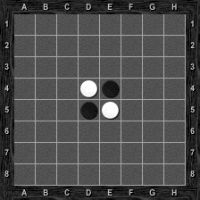
\includegraphics[scale=1]{images/board_start.jpg}
  }  
\end{figure}

Les joueurs posent des jetons de leur couleur à tour de rôle selon des
règles précises jusqu'à ce qu'aucun des deux ne puisse en mettre.
A la fin on compte le nombre de jeton de chaque joueur, et c'est celui qui en
a le plus qui gagne.

Le but du jeu est de capturer les jetons adverses afin de changer leur
couleur. La capture de pions survient lorsqu'un joueur place un de ses jetons
à l'extrémité d'un alignement de jetons adverses contigus et dont
l'autre extrémité est déjà occupée par un de ses propres
jetons. Le ou les pions \ embrassés par les deux jeton du joueur sont
capturés.


\begin{figure}[h]
  \caption {Capture de jetons}
  \noindent\makebox[\textwidth]{
    \centering
    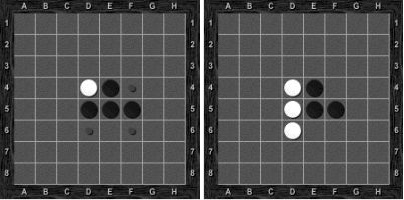
\includegraphics[width=\textwidth]{images/board_capture.png} 
  }
\end{figure}

Dans cet exemple on peut voir que le jour blanc peut mettre son jeton dans la
case F4, D6 ou G6. En mettant son jeton dans la case D6 il capture le jeton D5
qui devient noir.

\section{L'intelligence artificielle}

Pour ce travail nous voulons opposer un joueur (humain) à une machine
(intelligence artificielle). Pour cela, nous avons utilisé deux
méthodes pour guider les choix de la machine :

\subsection{Méthode aléatoire}

Dans cette méthode, la machine répond aux actions du joueur par des
choix de placements aléatoires parmi les positions possibles. Pour cela,
elle va choisir des cases du tablier de fa{\c c}on aléatoire et
vérifier si elles sont possibles en se basant sur les règles du jeu.
Cette méthode permet d'avoir l'illusion de jouer contre une machine, sauf
que cette machine n'est guidée par rien pour prendre sa décision et ne
peut être un adversaire efficace contre un joueur averti.

Pour rendre la machine plus intelligence il faut utiliser des méthodes
qui évalueraient chaque coup et maximiseraient la probabilité de
gagner. Une de ces méthodes consiste à utiliser l'algorithme minimax.

\subsection{Méthode du minimax}

La méthode du minimax est une technique de décision pour les jeux
à deux joueurs basée sur le théorème du Minimax de Von Neumann
dont l'objectif est de minimiser la perte maximale ou à l'inverse de
maximiser le gain minimal pour un joueur.

En se basant sur le théorème fondamental de la théorie des jeux
à deux joueurs, démontré en 1928 par John von Neumann. On sait que
pour tout jeu à deux joueurs et à information parfaite avec un nombre
fini de stratégies, il existe une évaluation V et une stratégie
mixte (Choix aléatoire parmi une liste de possibilités) telle que :

\tmtextit{\begin{enumeratealpha}
  \item Etant donné la stratégie du joueur A, le meilleur gain
  possible pour le joueur A est V, et
  
  \item Etant donné la stratégie du joueur B, le\tmtextit{} meilleur
  gain possible pour le joueur B est -V.
\end{enumeratealpha}}

On peut donc borner ses bénéfices et par la même occasion ceux de
son adversaire. L'idée est de maximiser le gain minimum en minimisant le
gain maximum de l'adversaire.

Avant d'aborder en détails l'algorithme du minimax, nous allons d'abord
expliquer quelques notions qui nous aiderons à mieux comprendre son
fonctionnement.

{\tmstrong{Les joueurs:}} Le joueur A est appelé Joueur Maximisant et le
joueur B est appelé Joueur Minimisant. Dans ce travaille le joueur
maximisant est l'ordinateur, puisque c'est lui qui va exécuter
l'algorithme et le joueur minimisant est son adversaire humain.

{\tmstrong{L'état du jeu: \tmtextmd{C'est une configuration possible du
jeu. Par exemple dans Othello un état représente la disposition des
jetons noirs et blancs dans l'Othellier. L'état initial représente
l'état du jeu avant qu'il ait commencé. Et les états terminaux
représentent les états qui mettent fin au jeu.}}}

\tmtextbf{Le fils d'un état ei:} noté f(ei), il représente les
états atteignables depuis ei.

\tmtextbf{L'arbre de jeu :}\tmtextbf{} C'est un arbre qui contient tous les
états possibles du jeu. La racine représente l'état initial, et
les feuilles représentent les états terminaux. Chaque noeud
intermédiaire représente une position de jeu et chaque arc le reliant
à son fils un coup possible permettant de passer à la position
représentée par ce fils. La figure 3 représente une partie de
l'arbre de jeu Othello engendré à partir de l'état initial.


\begin{figure}[h]
  \caption {Une partie de l'arbre de jeu de Othello}
  \noindent\makebox[\textwidth]{
    \centering
    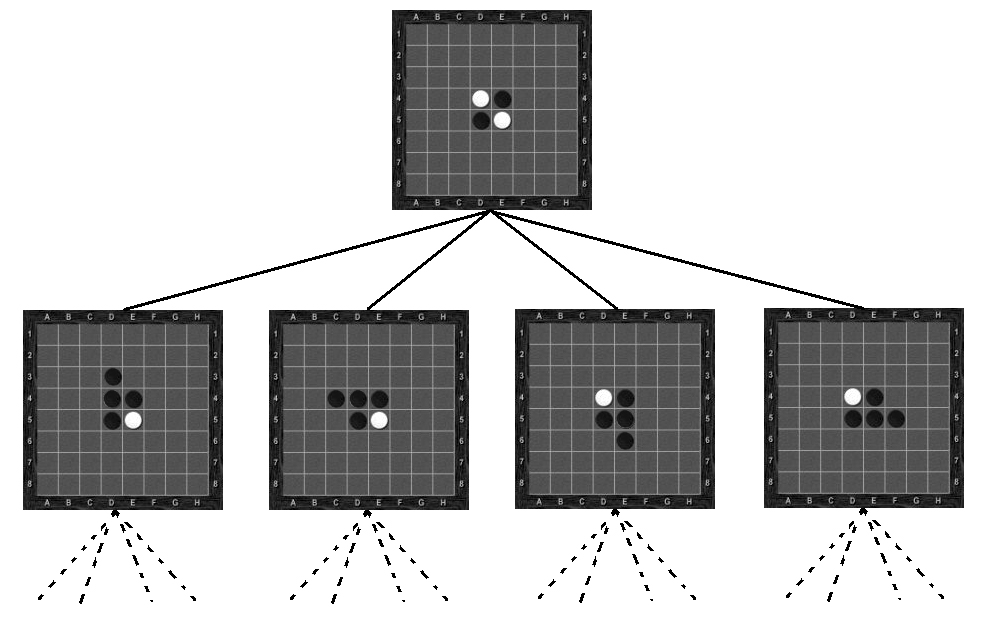
\includegraphics[width=\textwidth]{images/playing_tree.png} 
  }
\end{figure}



La génération de l'arbre de jeu est très couteuse parce que ce
dernier est généralement gigantesque. Par exemple le nombre total
d'états pour le jeu d'échecs est de 35\^{}100. Donc on ne peut pas
visiter tout l'arbre pour trouver les meilleurs coups à jouer.

- La fonction d'évaluation : Appelée aussi fonction heuristique, c'est
une fonction qui associe à chaque noeud une valeur estimant les gains du
coup pour le joueur maximisant. Par exemple, pour le jeu Othello plusieurs
fonctions d'évaluation peuvent être choisies. On peut utiliser une
matrice de valeurs tactiques associée aux cases pour avoir une fonction
d'évaluation plus performante. Le tableau qui suit représente une
matrice de valeurs tactiques en début de partie.

\begin{table}[h]
  \noindent\makebox[\textwidth]{
  \begin{tabular}{|c|c|c|c|c|c|c|c|}
    \hline
    500  & -150  &  30  &  10  &  10  &  30  & -150  &  500 \\
    \hline
    -150  &  -250  & 0 & 0 & 0 & 0 & -250 & -150\\
    \hline
    30 & 0 & 1 & 2 & 2 & 1 & 0 & 30\\
    \hline
    10 & 0 & 2 & 16 & 16 & 2 & 0 & 10\\
    \hline
    10 & 0 & 2 & 16 & 16 & 2 & 0 & 10\\
    \hline
    30 & 0 & 1 & 2 & 2 & 1 & 0 & 30\\
    \hline
    -150 & -250 & 0 & 0 & 0 & 0 & -250 & -150\\
    \hline
    500 & -150 & 30 & 10 & 10 & 30 & -150 & 500\\
    \hline
  \end{tabular}
  }
  \caption{Exemple de valeurs tactiques pour Othello}
\end{table}

Dans les valeurs tactiques ci-dessus, nous constatons que les coins de
l'othellier \ sont des positions très stratégiques puisque le gain
estimé est de 500. Ceci s'explique par le fait qu'un jeton sur cette case
est imprenable et offre la possibilité de capturer dans les mouvements
suivant le maximum de jetons sur 3 axes différents. Il est également
compréhensible que les cases qui entourent ces coins possèdent un gain
négatif puis qu'il laisse une chance à l'advesaire de le capturer.

Dans ce travail nous avons choisi de la pas considerer les valeurs tactiques
cela nécéssite une connaissance appronfondie du jeu pour faire
évoluer le tableau. Nous avous implémenté une fonction
d'évaluation qui fait la différence entre le nombre de jetons du
joueur et ceux de son adversaire. En plus d'être plus facile à
programmer cette fonction d'évaluation laisse une chance de gagner aux
joueurs non expérimentés comme nous.

\subsubsection{Algorithme du Minimax}

Le minimax est un algorithme pour la découverte de la solution optimale
dans un jeu à deux joueurs à information parfaite. Il effectue une
recherche en profondeur dans l'arbre de jeu pour décider du prochain coup
à jouer. L'exploration des neouds de cet arbre est limitée par un
paramètre de profondeur. Pour tout cela il est nécéssaire
d'utiliser :

\begin{itemizedot}
  \item Une fonction pour générer l'arbre de jeu, afin de
  déterminer les coups légaux à partir d'un état du jeu.
  
  \item Et une fonction heuristique pour évaluer un état de jeu.
\end{itemizedot}

à partir d'un état du jeu, l'algorithme visite l'arbre jusqu'à une
profondeur préalablement définie. Il évalue ensuite les feuilles
de l'arbre à l'aide de la fonction heuristique. Un score positif indique
une bonne position pour le joueur A et un score négatif une mauvaise
position, donc une bonne position pour le joueur B. Selon le joueur qui joue,
le passage d'un niveau à l'autre dans l'arbre est maximisant (pour le
joueur A) ou minimisant (pour le joueur B). Chaque joueur essaie de maximiser
son gain et de minimiser celui de son adversaire.

Le principe du minimax est de visiter l'arbre et de faire remonter la valeur
minimax à la racine. La valeur minimax est calculée récursivement
comme suit :

\begin{itemizedot}
  \tmtextit{\item Minimax(e) = h(e), si e est une feuille de l'arbre (jeu
  terminé).
  
  \item Minimax(e) = max (Minimax(e1), . . . , Minimax(en)), si e est un noeud
  Joueur \ \ \ \ \ \ (étape max)
  
  \item Minimax(e) = min (Minimax(e1), . . . , Minimax(en)), si e est un noeud
  Adversaire \ \ (étape min)}
\end{itemizedot}



\begin{algorithm}
  \caption{Algorithme Minimax}

  \begin{algorithmic}
  	\Statex\Require{Noeud e}
  	\Output{Valeur Minimax du noeud e}
    \Function{Minimax}{e}
      \If{final ?(e)}
        \Return h(e)
      \Else
        \If{joueur ?(e)}
	      \Return $max{Minimax(ei) \mid ei \in f(e)}$
	    \Else 
	      \Return $min{Minimax(ei) \mid ei \in f(e)}$
	    \EndIf
	  \EndIf
    \EndFunction
  \end{algorithmic}
\end{algorithm}



La figure 4 explique sur un exemple a deux niveaux le déroulement de
l'algorithme du minimax. On peut voir que la racine ne contient pas le gain le
plus élevé mais plutôt le maximum des pertes minimales. Donc
l'algorithme ne cherche pas le score le plus élevé mais plutôt le
gain le plus sûr.

\begin{figure}[H]
  \caption {Exemple de déroulement de l'algorithme Minimax}
  \noindent\makebox[\textwidth]{
    \centering
    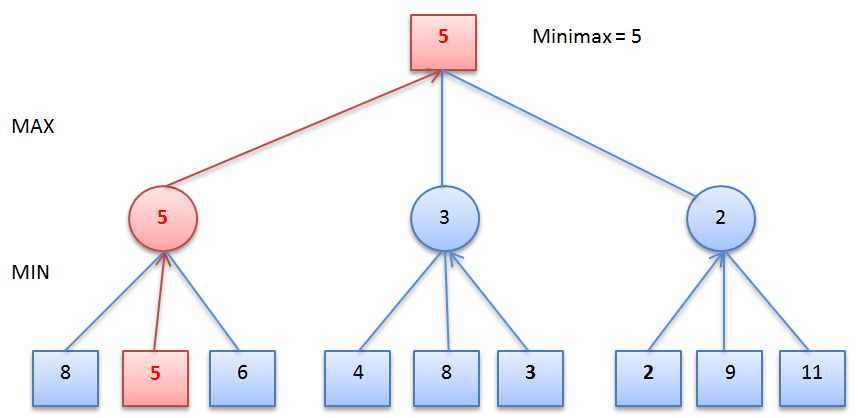
\includegraphics[width=\textwidth]{images/minimax_example.png} 
  }
\end{figure}

\tmtextbf{Propriétés de l'algorithme minimax}

Pour l'algorithme minimax la complexité en temps de est de O(b\^{}m) et
la complexité en espace est O(bm).Avec b = facteur de branchement et m =
est la profondeur de l'arbre. Nous n'avons pas pu avoir des chiffres pour
Othello mais par exemple pour les échecs b = 35 et m = 100.

\subsubsection{Problème d'espace et de temps de recherche}

Supposons qu'on veuille explorer tout l'arbre de jeu à partir de n'importe
quelle position. Cela permettrait de déterminer s'il existe un chemin
menant à la victoire, ou au moins au nul. Mais à cause du problème
de l'explosion combinatoire, la génération d'un tel arbre est trop
coûteuse pour être envisageable.

La première solution serait de limiter la profondeur d'exploration de
l'abre. Cela permettrait de réduire le nombre de coups et de réponses
à évaluer. Dans ce cas on atteint rarement les feuilles sauf en fin de
partie. Cette solution s'appelle le Minimax à profondeur limitée.

\subsubsection{Le Minimax à profondeur limitée}

C'est une variante de l'algorithme du minimax initial qui rajoute un indice de
profondeur afin de limiter la taille de l'arbre à générer. Le
principe de cette variante est de :

\tmtextit{\begin{itemizedot}
  \item Générer l'arbre de jeu jusqu'à une profondeur d à
  partir du noeud courant.
  
  \item Calculer la valeur de la fonction d'évaluation pour chaque noeud
  feuille, pas forcément terminal.
  
  \item Propager ces valeurs jusqu'aux noeuds non terminaux.
\end{itemizedot}}

\begin{algorithm}
  \caption{Algorithme Minimax à profondeur limitée}

  \begin{algorithmic}
  	\Statex\Require{Noeud e, Profondeur d}
  	\Output{Valeur Minimax du noeud e}
    \Function{Minimax}{e, d}
      \If{final ?(e) ou (d == 0)}
        \Return h(e)
      \Else
        \If{joueur ?(e)}
	      \Return $max{Minimax(ei, d-1) \mid ei \in f(e)}$
	    \Else 
	      \Return $min{Minimax(ei, d-1) \mid ei \in f(e)}$
	    \EndIf
	  \EndIf
    \EndFunction
  \end{algorithmic}
\end{algorithm}


{\tmstrong{Limites de l'algorithme Minimax à profondeur limitée}}

Si la profondeur de recherche est trop petite. Cela veut dire que l'algorithme cherche à déterminer les coups immédiats qui maximisent le score
du joueur A sans prévoir les coups de l'adversaire. La figure 5 montre le
déroulement de l'algorithme Minimax à profondeur limitée avec d=1.

\begin{figure}[h]
  \caption {Exemple de déroulement du Minimax à profondeur limitée avec d=1}
  \noindent\makebox[\textwidth]{
    \centering
    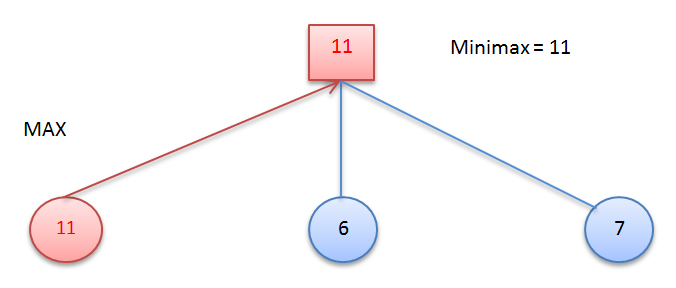
\includegraphics[width=\textwidth]{images/minimax_d1_example.png} 
  }
\end{figure}

On peut voir que le programme détermine les coups légaux, simule le
jeu et évalue chacun d'entre eux. Il décide ensuite que le coup avec
l'évaluation 11 est le meilleur et le propage au sommet. Cette
opération conduit le programme à choisir le coup avec l'évaluation
11 ce qui peut s'avérer être une décision désastreuse puisque
comme on peut le voir dans la figure 6, Le coup qui amenait à une position
immédiate de score 11, va en fait amener la position du jeu à un score
de -2. En effet si l'adversaire joue le coup qui mène vers
l'évaluation -2, alors le score final serait -2. On s'aper{\c c}oit alors
que le coup qui menait à l'évaluation 6 limite les dég{\^a}ts avec
un score de 1. Il sera donc préféré.

\begin{figure}[h]
  \caption {Exemple de déroulement du Minimax à profondeur limitée avec d=2}
  \noindent\makebox[\textwidth]{
    \centering
    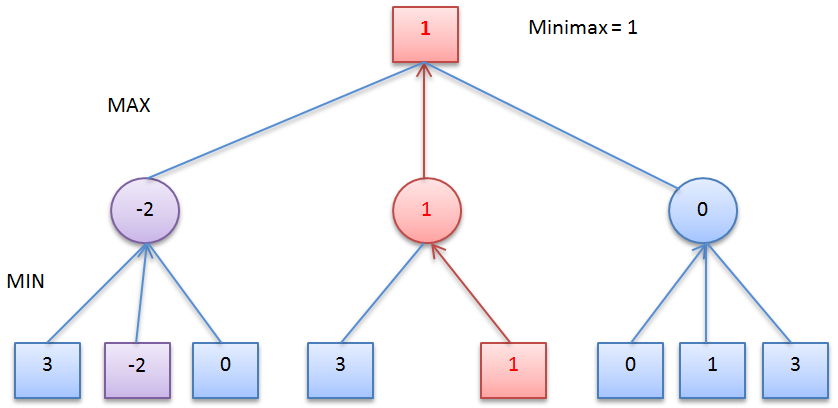
\includegraphics[width=\textwidth]{images/minimax_d2_example.png}
  }
\end{figure}

Le but est de maximiser la valeur de d pour prévoir le plus de coups
possibles à l'avance. Mais sans pour autant être confronté au
problème de l'explosion combinatoire. Pour cela on essaie d'élaguer
l'arbre de recherche. On peut noter que dans la figure 6, il n'est pas
nécessaire d'explorer toute la branche avec l'évaluation 0, puisque
cette dernière est inférieure à 1 (on cherche le max). Le calcul
des autres noeuds ne pourra pas améliorer la situation même si leurs
scores sont meilleures que 0. La variante Alpha Beta du Minimax utilise cet
élagage pour diminuer le nombre de branches à générer et
permettre par la même occasion d'augmenter la valeur de d.

\subsubsection{Le Minimax avec élagage {\tmem{Alpha Beta}}}

L'élagage Alpha Beta est une méthode permettant de réduire la
taille de l'arbre de jeu en élaguant les parties dont l'évaluation ne
contribue pas à celle de la racine. Cette méthode augmente de
manière significative les performances de l'algorithme Minimax sans
affecter le résultat. Pour élaguer certaines branches de l'arbre de
jeu on définit deux bornes $\alpha \nocomma \tmop{et} \beta$ tel que :

$\alpha$ représente de la borne inférieure de la valeur du noeud :
\begin{itemizedot}
  \item $\alpha$ = h(e) sur les feuilles, et initialisée à -$\infty$
  ailleurs.
  
  \item Dans les noeuds joueurs, $\alpha$ = MAX des valeurs obtenues sur les
  fils visités jusque-là.
  
  \item Dans les noeuds adversaires, elle est égale à la valeur
  $\alpha$ de son prédécesseur.
\end{itemizedot}
\ \ $\beta$ représente de la borne supérieure de la valeur du noeud :
\begin{itemizedot}
  \item $\beta$ = h(e) sur les feuilles, et initialisée à +$\infty$
  ailleurs.
  
  \item Dans les noeuds adversaires, $\beta$ = MIN des valeurs obtenues sur
  les fils visités jusque-là.
  
  \item Dans les noeuds joueurs elle est égale à la valeur $\beta$ de
  son prédécesseur.
\end{itemizedot}
Pour Othello, nous avons remplacé les valeurs -$\infty$ et +$\infty$
respectivement par les valeurs -64 et + 64, puisque dans Othello la
différence max entre les jetons des joueurs (fonction heuristique) ne peut
dépasser 64. Les noeuds élagués sont ceux tel que

\ \ \ \ \ \ \ \ \ \ \ \ \ \ \ \ \ \ \ \ \ \ \ \ \ \ \ \ \ \ \ \ \ \ \ \ \ \ \
\ \ \ \ \ \ \ $ H ( e) \in [ \tmmathbf{\beta} \nocomma \nocomma,
\tmmathbf{\alpha}] \tmop{et} \tmmathbf{\alpha} \geqslant \tmmathbf{\beta}$

Donc l'alpha-coupure intervient dans un noeud adversaire (MIN) lorsque sa
beta-valeur est inférieure à l'alpha-valeur de son parent. Et la
beta-coupure intervient dans un noeud joueur (MAX) lorsque sa alpha-valeur est supérieure à la beta-valeur de son parent.

\begin{figure}[h]
  \caption {Exemples de coupures alpha et beta}
  \noindent\makebox[\textwidth]{
    \centering
    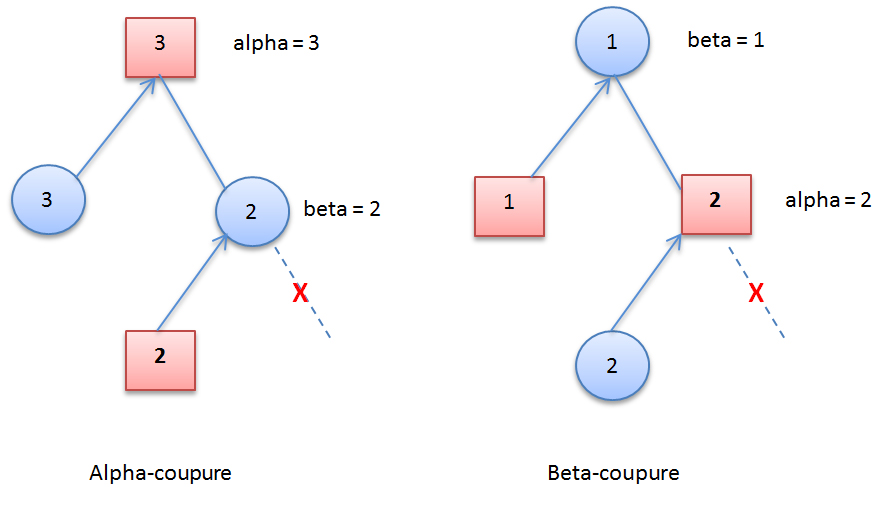
\includegraphics[width=\textwidth]{images/minimax_ab_example.png}
  }
\end{figure}

\begin{algorithm}
  \caption{Algorithme Minimax avec élagage $\alpha \beta$}

  \begin{algorithmic}
  	\Statex\Require{Noeud e, Profondeur d, Alpha $\alpha$, Beta $\beta$}
  	\Output{Valeur Minimax du noeud e}
    \Function{Minimax}{e, d, }
      \If{final ?(e) ou (d == 0)}
        \Return h(e)
      \Else
        \If{joueur ?(e)}
          \State $v = -\infty$
          \For{$fi \in f(e)$}
            \State $v = max(v, Minimax(fi, d-1, \alpha, \beta))$
            \If{$v > \beta$} \Return v \EndIf
            \State $\alpha = max(\alpha, v)$
          \EndFor
	    \Else 
          \State $v = +\infty$
          \ForAll{$fi \in f(e)$}
            \State $v = min(v, Minimax(fi, d-1, \alpha, \beta))$
            \If{$v > \alpha$} \Return v \EndIf
            \State $\beta = min(\beta, v)$
          \EndFor
	    \EndIf
	  \EndIf
    \EndFunction
  \end{algorithmic}
\end{algorithm}

Dans la figure suivante nous observons l'exécution de l'algorithme du
minimax avec élagage alpha beta sur l'arbre de jeu vu dans la figure 6.


\begin{figure}[h]
  \caption {Exemple de déroulement de l'algorithme minimax alpha-beta avec d = 2}
  \noindent\makebox[\textwidth]{
    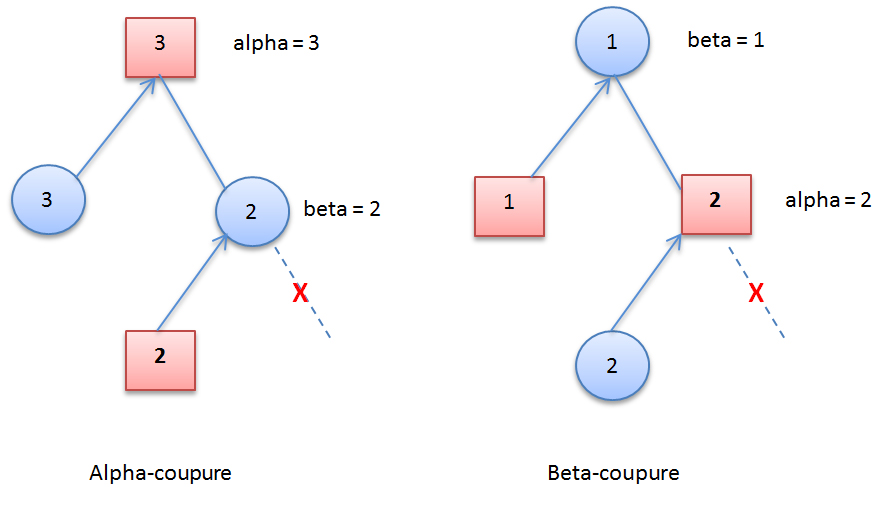
\includegraphics[width=\textwidth]{images/minimax_ab_example.png}
  }
\end{figure}

On peut observer que le résultat reste le même que celui obtenu en
appliquant l'algorithme du minimax classique. Mais l'élagage alpha beta a
permis de ne pas visiter les dernières branches, ce qui augmente les
performances de l'algorithme et nous permet par la même occasion
d'augmenter la profondeur d'exploration du graphe. L'ordre d'apparition des
noeuds influence beaucoup le rendement de l'élagage. Examiner d'abord les
noeuds à forte valeur d'évaluation maximise le rendement de
l'algorithme.

La complexité en temps de l'algorithme minimax avec élagage alpha beta
revient dans le meilleur des cas à O(b\^{}(m/2)). Cela permet d'augmenter
la profondeur de recherche pour améliorer les résultats sans trop
affecter les performances. Et dans le pire des cas elle est identique à
celle du minimax.


\section{Implémentation}

Dans cette partie nous allons détailler les étapes d'implémentation de l'application. 

\subsection{Compilation}

Afin de générer les fichiers binaires, nous avons créé un Makefile très générique paramétrable à souhait. Il semblerait que les performances d'exécution soit optimisées en utilisant le compilateur ocamlopt. Ce qui rend le choix intéressant  dans un cas d'utilisation comme le nôtre ou le programme est sujet à des explosions combinatoires. 

Pour une compilation standard avec \texttt{ocamlc}, utiliser : \texttt{make}

\begin{figure}[H]
\caption{Utilisation du Makefile}
\begin{verbatim}
# Pour recompiler le système progressivement :
#     make
# Pour recalculer les dépendances entre les modules :
#     make depend
# Pour supprimer l'exécutable et les fichiers compilés :
#     make clean
# Pour compiler avec le compileur de code natif
#     make opt
\end{verbatim}
\end{figure}

\subsection{Utilisation}

Afin de lancer l'application, tapez: \texttt{./othello}

Il est possible de spécifier des arguments à l'exécutable qui vont influencer le déroulement du jeu. Vous pouvez obtenir la liste ces options avec :

\begin{figure}[H]
\caption{Utilisation de l'exécutable}
\begin{verbatim}
$ ./othello --help
othello
  -size <int> : Taille d'une case en pixels
  -ia <bool> : Intelligence artificielle on/off
               | true  -> Minimax ab 
               | false -> Case aléatoire
  -depth <int> : Profondeur maximale d'exploration 
                 de l'arbre des possibilités Minimax 
  -background <int> <int> <int> : Couleur du fond (RGB)
  -help : Afficher cette liste d'options
  --help : Afficher cette liste d'options
\end{verbatim}
\end{figure}

Les options par défaut de l'application sont :

\begin{figure}[H]
\caption{Configuration par défaut}
{\scriptsize\noindent
\begin{longtable}{r|l}
\mlcodeline{1}{\mlkeyword{val}~cell\_{}size~\mloperator{\mbox{\COLON}}~int~ref~\mlkeyword{=}~\mloperator{\{}contents~\mlkeyword{=}~50\mloperator{\}}
}
\mlcodeline{2}{\mlkeyword{val}~bg\_{}r~\mloperator{\mbox{\COLON}}~int~ref~\mlkeyword{=}~\mloperator{\{}contents~\mlkeyword{=}~50\mloperator{\}}
}
\mlcodeline{3}{\mlkeyword{val}~bg\_{}g~\mloperator{\mbox{\COLON}}~int~ref~\mlkeyword{=}~\mloperator{\{}contents~\mlkeyword{=}~150\mloperator{\}}
}
\mlcodeline{4}{\mlkeyword{val}~bg\_{}b~\mloperator{\mbox{\COLON}}~int~ref~\mlkeyword{=}~\mloperator{\{}contents~\mlkeyword{=}~50\mloperator{\}}
}
\mlcodeline{5}{\mlkeyword{val}~size~\mloperator{\mbox{\COLON}}~int~ref~\mlkeyword{=}~\mloperator{\{}contents~\mlkeyword{=}~8\mloperator{\}}
}
\mlcodeline{6}{\mlkeyword{val}~ia~\mloperator{\mbox{\COLON}}~bool~ref~\mlkeyword{=}~\mloperator{\{}contents~\mlkeyword{=}~\mlkeywordB{true}\mloperator{\}}
}
\mlcodeline{7}{\mlkeyword{val}~depth~\mloperator{\mbox{\COLON}}~int~ref~\mlkeyword{=}~\mloperator{\{}contents~\mlkeyword{=}~4\mloperator{\}}
}
\end{longtable}
}
\end{figure}

\subsection{Algorithmes notables}

\subsubsection{Direction légale}

Cette méthode permet de déterminer si une direction de jeu est légale. À partir d'un case donnée, l'algorithme récursif initie la direction comme illégale. En regardant le premier voisin dans la direction donnée, la case doit contenir impérativement un jeton du joueur opposé. L'itération récursive continue alors en indiquant grâce à un booléen qu'au moins un jeton de l'adversaire est dans l'alignement. Lorsqu'un jeton de couleur de joueur est identifié, l'algorithme s'arrête et la direction est jouable. Si une case vide est rencontrée, la direction n'est pas légale.

\begin{figure}[H]
\caption{Direction légale}
{\scriptsize\noindent
\begin{longtable}{r|l}
\mlcodeline{1}{\mlcomments{(*~Methode~de~test~de~direction~légale~*)}
}
\mlcodeline{2}{\mlkeywordA{let}~playable\_{}dir~board~c~(x\mloperator{\mbox{,}}~y)~(dx\mloperator{\mbox{,}}~dy)~\mlkeyword{=}
}
\mlcodeline{3}{~~\mlkeywordA{let~rec}~playable\_{}dir\_{}rec~(x\mloperator{\mbox{,}}~y)~valid~\mlkeyword{=}
}
\mlcodeline{4}{~~~~\mlkeyword{if}~not~(check\_{}pos~board~x~y)~\mlkeyword{then}
}
\mlcodeline{5}{~~~~~~\mlkeywordB{false}
}
\mlcodeline{6}{~~~~\mlkeyword{else}~(
}
\mlcodeline{7}{~~~~~~\mlkeyword{match}~board\mloperator{.}(x)\mloperator{.}(y)~\mlkeyword{with}
}
\mlcodeline{8}{~~~~~~~~\mloperator{|}~Empty~\mlkeyword{->}~\mlkeywordB{false}
}
\mlcodeline{9}{~~~~~~~~\mloperator{|}~cell~\mlkeyword{->}
}
\mlcodeline{10}{~~~~~~~~~~\mlkeyword{if}~cell~\mlkeyword{=}~(get\_{}opponent~c)~\mlkeyword{then}
}
\mlcodeline{11}{~~~~~~~~~~~~playable\_{}dir\_{}rec~(x~\mloperator{+}~dx\mloperator{\mbox{,}}~y~\mloperator{+}~dy)~\mlkeywordB{true}
}
\mlcodeline{12}{~~~~~~~~~~\mlkeyword{else}
}
\mlcodeline{13}{~~~~~~~~~~~~valid
}
\mlcodeline{14}{~~~~)
}
\mlcodeline{15}{~~~~\mlkeywordA{in}~playable\_{}dir\_{}rec~(x~\mloperator{+}~dx\mloperator{\mbox{,}}~y~\mloperator{+}~dy)~\mlkeywordB{false}
}
\mlcodeline{16}{\mloperator{\mbox{\SC}\mbox{\SC}}}
\end{longtable}
}
\end{figure}


\subsubsection{Coup Légal}

Afin de déterminer si un coup est légal, cet algorithme va tester si parmi les 8 directions possibles de capture, au moins l'une d'être est jouable. Pour ce faire et à partir de la liste des directions donnée, un fold-left testera chacune d'entre elles et comparera leur légalité grâce a un simple prédicat. Nous aurions pu optimiser légèrement cette function en utilisant notre fonction 'fold-until' décrit dans la section 'Implémentation Minimax Alpha Beta' et stopper le test des directions à partir du moment où l'une d'entre elle est légale.

\begin{figure}[H]
\caption{Coup légal}
{\scriptsize\noindent
\begin{longtable}{r|l}
\mlcodeline{1}{\mlcomments{(*~Methode~de~test~de~coup~légal~{=>\mbox{}}~Vrai~si~le~coup~est~légal~*)}
}
\mlcodeline{2}{\mlkeywordA{let}~playable\_{}cell~board~c~x~y~\mlkeyword{=}
}
\mlcodeline{3}{~~\mlkeyword{if}~not~(check\_{}pos~board~x~y)~\mlkeyword{then}
}
\mlcodeline{4}{~~~~\mlkeywordB{false}
}
\mlcodeline{5}{~~\mlkeyword{else}~(
}
\mlcodeline{6}{~~~~\mlkeywordA{let}~directions~\mlkeyword{=}~\mloperator{[}~
}
\mlcodeline{7}{~~~~~~\mloperator{(-}1\mloperator{\mbox{,}}~-1)\mloperator{\mbox{\SC}}~\mloperator{(-}1\mloperator{\mbox{,}}~0)\mloperator{\mbox{\SC}}~\mloperator{(-}1\mloperator{\mbox{,}}~1)\mloperator{\mbox{\SC}}~
}
\mlcodeline{8}{~~~~~~(0~\mloperator{\mbox{,}}~-1)\mloperator{\mbox{\SC}}~\mlcomments{(*~X~*)}~~(0~\mloperator{\mbox{,}}~1)\mloperator{\mbox{\SC}}~
}
\mlcodeline{9}{~~~~~~(1~\mloperator{\mbox{,}}~-1)\mloperator{\mbox{\SC}}~(1~\mloperator{\mbox{,}}~0)\mloperator{\mbox{\SC}}~(1~\mloperator{\mbox{,}}~1)~
}
\mlcodeline{10}{~~~~\mloperator{]}
}
\mlcodeline{11}{~~~~\mlkeywordA{in}~\mlkeyword{match}~board\mloperator{.}(x)\mloperator{.}(y)~\mlkeyword{with}
}
\mlcodeline{12}{~~~~~~\mloperator{|}~Empty~\mlkeyword{->}~(~\mlkeywordB{true}~\mloperator{\&\&}~(	
}
\mlcodeline{13}{		~~~~\mlmodulename{List}\mbox{}\mloperator{.}fold\_{}left
}
\mlcodeline{14}{		~~~~~~(\mlkeyword{fun}~a~b~\mlkeyword{->}~a~\mloperator{||}~b)~
}
\mlcodeline{15}{		~~~~~~\mlkeywordB{false}
}
\mlcodeline{16}{~~~~~~~~~~~~~~(\mlmodulename{List}\mbox{}\mloperator{.}map
}
\mlcodeline{17}{~~~~~~~~~~~~~~~~(\mlkeyword{fun}~d~\mlkeyword{->}~playable\_{}dir~board~c~(x\mloperator{\mbox{,}}~y)~d)
}
\mlcodeline{18}{~~~~~~~~~~~~~~~~directions	
}
\mlcodeline{19}{~~~~~~~~~~~~~~)
}
\mlcodeline{20}{~~~~~~~~~~~~)
}
\mlcodeline{21}{~~~~~~~~~~)~
}
\mlcodeline{22}{~~~~~~~\mloperator{|}~\mloperator{\_}~\mlkeyword{->}~\mlkeywordB{false}	
}
\mlcodeline{23}{~~)
}
\mlcodeline{24}{\mloperator{\mbox{\SC}\mbox{\SC}}}
\end{longtable}
}
\end{figure}

\subsubsection{Simulation de jeu}

Cette méthode permet la simulation d'un coup joué. Tout premièrement, l'algorithme va copier l'état du tablier et la position des jeton. Le tableau contenant uniquement des références sur jetons (type cell), il nous est impossible de copier le tableau via un Array.copy par example, puisque les références copiées pointerons toujours sur les même objets de case. Nous  utiliserons donc une fonction customisée de copy de tableau. L'algorithme récursif de capture des jetons est très similaire à celle vu précédemment. La fonction retourne le plateau de jeu à l'état suivant le coup simulé.

\begin{figure}[H]
\caption{Simuler un coup}
{\scriptsize\noindent
\begin{longtable}{r|l}
\mlcodeline{1}{\mlcomments{(*~Méthode~pour~simuler~le~jeu~sur~une~case~*)}
}
\mlcodeline{2}{\mlkeywordA{let}~sim\_{}play\_{}cell~board~c~x~y~\mlkeyword{=}
}
\mlcodeline{3}{~~\mlkeywordA{let}~sim\_{}board~\mlkeyword{=}~(copy\_{}board~board)~\mlkeywordA{in}
}
\mlcodeline{4}{~~\mlkeywordA{let}~directions~\mlkeyword{=}~\mloperator{[}~
}
\mlcodeline{5}{~~~~\mloperator{(-}1\mloperator{\mbox{,}}~-1)\mloperator{\mbox{\SC}}~\mloperator{(-}1\mloperator{\mbox{,}}~0)\mloperator{\mbox{\SC}}~\mloperator{(-}1\mloperator{\mbox{,}}~1)\mloperator{\mbox{\SC}}~
}
\mlcodeline{6}{~~~~(0~\mloperator{\mbox{,}}~-1)\mloperator{\mbox{\SC}}~\mlcomments{(*~X~*)}~~(0~\mloperator{\mbox{,}}~1)\mloperator{\mbox{\SC}}~
}
\mlcodeline{7}{~~~~(1~\mloperator{\mbox{,}}~-1)\mloperator{\mbox{\SC}}~(1~\mloperator{\mbox{,}}~0)\mloperator{\mbox{\SC}}~(1~\mloperator{\mbox{,}}~1)~
}
\mlcodeline{8}{~~\mloperator{]}
}
\mlcodeline{9}{~~\mlkeywordA{and}~opponent~\mlkeyword{=}~(get\_{}opponent~c)~
}
\mlcodeline{10}{~~\mlkeywordA{in}~(
}
\mlcodeline{11}{~~~~\mlmodulename{List}\mbox{}\mloperator{.}iter~											
}
\mlcodeline{12}{~~~~~~(\mlkeyword{fun}~(dx\mloperator{\mbox{,}}~dy)~\mlkeyword{->}
}
\mlcodeline{13}{~~~~~~~~\mlkeyword{if}~(playable\_{}dir~sim\_{}board~c~(x\mloperator{\mbox{,}}~y)~(dx\mloperator{\mbox{,}}~dy))~\mlkeyword{then}
}
\mlcodeline{14}{~~~~~~~~~~\mlkeywordA{let~rec}~take~(x\mloperator{\mbox{,}}~y)~\mlkeyword{=}
}
\mlcodeline{15}{~~~~~~~~~~~~\mlkeyword{if}~(check\_{}pos~sim\_{}board~x~y)~\mlkeyword{then}	
}
\mlcodeline{16}{~~~~~~~~~~~~\mlkeyword{if}~(sim\_{}board\mloperator{.}(x)\mloperator{.}(y)~\mlkeyword{=}~opponent)~\mlkeyword{then}~(
}
\mlcodeline{17}{~~~~~~~~~~~~~~sim\_{}board\mloperator{.}(x)\mloperator{.}(y)~\mloperator{<\mbox{}-}~c\mloperator{\mbox{\SC}}
}
\mlcodeline{18}{~~~~~~~~~~~~~~take~(x~\mloperator{+}~dx\mloperator{\mbox{,}}~y~\mloperator{+}~dy)
}
\mlcodeline{19}{~~~~~~~~~~~~)
}
\mlcodeline{20}{~~~~~~~~~~\mlkeywordA{in}~take~(x~\mloperator{+}~dx\mloperator{\mbox{,}}~y~\mloperator{+}~dy)
}
\mlcodeline{21}{~~~~~~)
}
\mlcodeline{22}{~~~~~~directions
}
\mlcodeline{23}{~~)\mloperator{\mbox{\SC}}~
}
\mlcodeline{24}{~~sim\_{}board\mloperator{.}(x)\mloperator{.}(y)~\mloperator{<\mbox{}-}~c\mloperator{\mbox{\SC}}
}
\mlcodeline{25}{~~sim\_{}board
}
\mlcodeline{26}{\mloperator{\mbox{\SC}\mbox{\SC}}}
\end{longtable}
}
\end{figure}


\subsubsection{Algorimthe Minimax \tmem{Alpha Beta}}

Dans une premier temps, le langage OCAML ne permettant pas d'interrompre l'éxecution d'une boucle directement via des instructions telles que 'break','return', nous avons du créér une fonction récursive (figure 15) permettant d'itérer à travers une liste d'élément en intégrant un accumulateur et un callback. L'itération s'arrêtera lorsqu'un prédicat [p] sur l'accumulateur sera validé.

\begin{figure}[h]
\caption{Fonction récursive fold\_until}
{\scriptsize\noindent\begin{longtable}{r|l}
\mlcodeline{1}{\mlcomments{(**~Méthode~récursive~de~Fold~left~sur~une~liste~avec~la~{function}~{[}f{]}~
}}
\mlcodeline{2}{\mlcomments{~~~jusqu'à~que~ce~que~le~prédicat~{[}p{]}~soit~satisfait~*)}
}
\mlcodeline{3}{\mlkeywordA{let~rec}~fold\_{}until~f~p~acc~l~\mlkeyword{=}~
}
\mlcodeline{4}{~~\mlkeyword{match}~l~\mlkeyword{with}
}
\mlcodeline{5}{~~\mloperator{|}~t~\mloperator{\mbox{\COLON}\mbox{\COLON}}~q~\mlkeyword{when}~p~acc~\mlkeyword{->}~acc				
}
\mlcodeline{6}{~~\mloperator{|}~t~\mloperator{\mbox{\COLON}\mbox{\COLON}}~q~\mlkeyword{->}~fold\_{}until~f~p~(f~acc~t)~q
}
\mlcodeline{7}{~~\mloperator{|}~\mloperator{[}\mloperator{]}~\mlkeyword{->}~acc
}
\mlcodeline{8}{\mloperator{\mbox{\SC}\mbox{\SC}}
}
\mlcodeline{9}{\mlcomments{(**~Retourne~l'accumulateur~*)}}
\end{longtable}
}
\end{figure}

Nous pourrons alors facilement implémenter l'algorithme Minimax $\alpha \beta$ détaillé précédemment.

\begin{figure}[H]
\caption{Implémentation de l'algorithme minimax $\alpha \beta$}
{\scriptsize\noindent\begin{longtable}{r|l}
\mlcodeline{1}{\mlcomments{(**~Méthode~récursive~de~calcul~alphabeta~des~noeuds~de~l'arbre~*)}
}
\mlcodeline{2}{\mlkeywordA{let~rec}~alpha\_{}beta~board~c~d~a~b~\mlkeyword{=}
}
\mlcodeline{3}{~~\mlkeyword{if}~(is\_{}finished~board~\mlkeyword{or}~d~\mlkeyword{=}~0)~\mlkeyword{then}
}
\mlcodeline{4}{~~~~score~board~White
}
\mlcodeline{5}{~~\mlkeyword{else}~\mlkeywordA{let}~playable\_{}cells~\mlkeyword{=}~playable\_{}cells~board~c~\mlkeywordA{in}~
}
\mlcodeline{6}{~~~~\mlkeyword{match}~c~\mlkeyword{with}
}
\mlcodeline{7}{~~~~\mloperator{|}~White~\mlkeyword{->}~\mlkeywordA{let}~a2~\mlkeyword{=}~ref~a~\mlkeywordA{in}
}
\mlcodeline{8}{~~~~~~~~fold\_{}until~
}
\mlcodeline{9}{~~~~~~~~~~(
}
\mlcodeline{10}{~~~~~~~~~~~~\mlkeyword{fun}~v~(x\mloperator{\mbox{,}}~y)~\mlkeyword{->}~
}
\mlcodeline{11}{~~~~~~~~~~~~~~\mlkeywordA{let}~ab~\mlkeyword{=}~alpha\_{}beta~
}
\mlcodeline{12}{~~~~~~~~~~~~~~~~(sim\_{}play\_{}cell~board~c~x~y)~
}
\mlcodeline{13}{~~~~~~~~~~~~~~~~Black~
}
\mlcodeline{14}{~~~~~~~~~~~~~~~~(d~\mloperator{-}~1)~
}
\mlcodeline{15}{~~~~~~~~~~~~~~~~\mloperator{\mbox{}\hspace{0pt}{!}\hspace{0pt}}a2~b~\mlkeywordA{in}
}
\mlcodeline{16}{~~~~~~~~~~~~~~\mlkeywordA{let}~v2~\mlkeyword{=}~max~v~ab~\mlkeywordA{in}
}
\mlcodeline{17}{~~~~~~~~~~~~~~a2~\mloperator{\mbox{\COLON}{}=}~max~v2~\mloperator{\mbox{}\hspace{0pt}{!}\hspace{0pt}}a2\mloperator{\mbox{\SC}}
}
\mlcodeline{18}{~~~~~~~~~~~~~~v2
}
\mlcodeline{19}{~~~~~~~~~~)	
}
\mlcodeline{20}{~~~~~~~~~~(\mlkeyword{fun}~v~\mlkeyword{->}~v~\mloperator{>\mbox{}}~b)~
}
\mlcodeline{21}{~~~~~~~~~~\mloperator{(-}((\mlmodulename{Array}\mbox{}\mloperator{.}length~board)~\mloperator{*}~(\mlmodulename{Array}\mbox{}\mloperator{.}length~board\mloperator{.}(0))))
}
\mlcodeline{22}{~~~~~~~~~~playable\_{}cells
}
\mlcodeline{23}{~~~~\mloperator{|}~\mloperator{\_}~\mlkeyword{->}~\mlkeywordA{let}~b2~\mlkeyword{=}~ref~b~\mlkeywordA{in}
}
\mlcodeline{24}{~~~~~~~~fold\_{}until~
}
\mlcodeline{25}{~~~~~~~~~~(
}
\mlcodeline{26}{~~~~~~~~~~~~\mlkeyword{fun}~v~(x\mloperator{\mbox{,}}~y)~\mlkeyword{->}~
}
\mlcodeline{27}{~~~~~~~~~~~~~~\mlkeywordA{let}~ab~\mlkeyword{=}~alpha\_{}beta~
}
\mlcodeline{28}{~~~~~~~~~~~~~~~~(sim\_{}play\_{}cell~board~c~x~y)~
}
\mlcodeline{29}{~~~~~~~~~~~~~~~~White~
}
\mlcodeline{30}{~~~~~~~~~~~~~~~~(d~\mloperator{-}~1)~
}
\mlcodeline{31}{~~~~~~~~~~~~~~~~a~\mloperator{\mbox{}\hspace{0pt}{!}\hspace{0pt}}b2~\mlkeywordA{in}
}
\mlcodeline{32}{~~~~~~~~~~~~~~\mlkeywordA{let}~v2~\mlkeyword{=}~min~v~ab~\mlkeywordA{in}
}
\mlcodeline{33}{~~~~~~~~~~~~~~b2~\mloperator{\mbox{\COLON}{}=}~min~v2~\mloperator{\mbox{}\hspace{0pt}{!}\hspace{0pt}}b2\mloperator{\mbox{\SC}}
}
\mlcodeline{34}{~~~~~~~~~~~~~~v2
}
\mlcodeline{35}{~~~~~~~~~~)	
}
\mlcodeline{36}{~~~~~~~~~~(\mlkeyword{fun}~v~\mlkeyword{->}~v~\mloperator{<\mbox{}}~a)~
}
\mlcodeline{37}{~~~~~~~~~~((\mlmodulename{Array}\mbox{}\mloperator{.}length~board)~\mloperator{*}~(\mlmodulename{Array}\mbox{}\mloperator{.}length~board\mloperator{.}(0)))
}
\mlcodeline{38}{~~~~~~~~~~~playable\_{}cells
}
\mlcodeline{39}{\mloperator{\mbox{\SC}\mbox{\SC}}}
\end{longtable}
}

\end{figure}

\subsubsection{Algorithme: Tour de la machine de jouer}

Cette méthode décrit le tour de la machine. À partir de la liste des coûts immédiats, l'algorithme va évaluer chacun d'entre eux grâce à l'algorithme Minimax $\alpha \beta$. Les coup sont alors pondérés et la fonction récursive va retourner le meilleur mouvement à faire. Le programme va alors jouer la case grâces au coordonnées de la position de cette dernière.

\begin{figure}[h]
\caption{Méthode pour le tour de la machine}

{\scriptsize\noindent\begin{longtable}{r|l}
\mlcodeline{1}{\mlcomments{(**~Methode{\mbox{\COLON}}~Tour~de~la~machine~intelligente~*)}
}
\mlcodeline{2}{\mlkeywordA{let}~ia\_{}turn~board~\mlkeyword{=}~
}
\mlcodeline{3}{~~\mlkeywordA{let}~playable\_{}cells~\mlkeyword{=}~playable\_{}cells~board~White~\mlkeywordA{in}~
}
\mlcodeline{4}{~~~~\mlkeyword{match}~(\mlmodulename{List}\mbox{}\mloperator{.}length~playable\_{}cells)~\mlkeyword{with}
}
\mlcodeline{5}{~~~~\mloperator{|}~0~\mlkeyword{->}~()
}
\mlcodeline{6}{~~~~\mloperator{|}~\mloperator{\_}~\mlkeyword{->}~
}
\mlcodeline{7}{~~~~~~(\mlkeywordA{let}~x\mloperator{\mbox{,}}~y~\mlkeyword{=}
}
\mlcodeline{8}{~~~~~~~~\mlkeywordA{let~rec}~get\_{}best\_{}move~ab~cell~playable\_{}cells~\mlkeyword{=}
}
\mlcodeline{9}{~~~~~~~~~~\mlkeyword{match}~playable\_{}cells~\mlkeyword{with}
}
\mlcodeline{10}{~~~~~~~~~~\mloperator{|}~(x\mloperator{\mbox{,}}~y)~\mloperator{\mbox{\COLON}\mbox{\COLON}}~q~\mlkeyword{->}~
}
\mlcodeline{11}{~~~~~~~~~~~~\mlkeywordA{let}~a~\mlkeyword{=}~\mloperator{-}((\mlmodulename{Array}\mbox{}\mloperator{.}length~board)~\mloperator{*}~(\mlmodulename{Array}\mbox{}\mloperator{.}length~board\mloperator{.}(0)))
}
\mlcodeline{12}{~~~~~~~~~~~~\mlkeywordA{and}~b~\mlkeyword{=}~((\mlmodulename{Array}\mbox{}\mloperator{.}length~board)~\mloperator{*}~(\mlmodulename{Array}\mbox{}\mloperator{.}length~board\mloperator{.}(0)))
}
\mlcodeline{13}{~~~~~~~~~~~~\mlkeywordA{and}~old\_{}ab~\mlkeyword{=}~ab~\mlkeywordA{in}~
}
\mlcodeline{14}{~~~~~~~~~~~~~~\mlkeywordA{let}~ab~\mlkeyword{=}~(
}
\mlcodeline{15}{~~~~~~~~~~~~~~alpha\_{}beta~
}
\mlcodeline{16}{~~~~~~~~~~~~~~~~(sim\_{}play\_{}cell~board~White~x~y)~
}
\mlcodeline{17}{~~~~~~~~~~~~~~~~Black~
}
\mlcodeline{18}{~~~~~~~~~~~~~~~~\mloperator{(\mbox{}\hspace{0pt}{!}\hspace{0pt}}depth~\mloperator{-}~1)~
}
\mlcodeline{19}{~~~~~~~~~~~~~~~~a~b
}
\mlcodeline{20}{~~~~~~~~~~~~~~)~\mlkeywordA{in}
}
\mlcodeline{21}{~~~~~~~~~~~~~~~~\mlkeyword{if}~ab~\mloperator{>\mbox{}}~old\_{}ab~\mlkeyword{then}~get\_{}best\_{}move~ab~(x\mloperator{\mbox{,}}~y)~q~
}
\mlcodeline{22}{~~~~~~~~~~~~~~~~\mlkeyword{else}~get\_{}best\_{}move~old\_{}ab~cell~q
}
\mlcodeline{23}{~~~~~~~~~~\mloperator{|}~\mloperator{[}\mloperator{]}~\mlkeyword{->}~cell
}
\mlcodeline{24}{~~~~~~~~\mlkeywordA{in}~get\_{}best\_{}move~
}
\mlcodeline{25}{~~~~~~~~~~\mloperator{(-}((\mlmodulename{Array}\mbox{}\mloperator{.}length~board)~\mloperator{*}~(\mlmodulename{Array}\mbox{}\mloperator{.}length~board\mloperator{.}(0))))~
}
\mlcodeline{26}{~~~~~~~~~~(\mlmodulename{List}\mbox{}\mloperator{.}hd~playable\_{}cells)~
}
\mlcodeline{27}{~~~~~~~~~~(\mlmodulename{List}\mbox{}\mloperator{.}tl~playable\_{}cells)
}
\mlcodeline{28}{~~~~~~\mlkeywordA{in}~play\_{}cell~board~White~x~y)
}
\mlcodeline{29}{\mloperator{\mbox{\SC}\mbox{\SC}}}
\end{longtable}
}

\end{figure}

\newpage

\section{Module {\tt{Othello}} : Documentation}
\label{module:Othello}\index{Othello@\verb`Othello`}




\ocamldocvspace{0.5cm}



\label{val:Othello.cell-underscoresize}\begin{ocamldoccode}
val cell_size : int Pervasives.ref
\end{ocamldoccode}
\index{cell-underscoresize@\verb`cell_size`}
\begin{ocamldocdescription}
Définition de la largeur des cellules en pixels


\end{ocamldocdescription}




Défaut: 75



\label{val:Othello.bg-underscorer}\begin{ocamldoccode}
val bg_r : int Pervasives.ref
\end{ocamldoccode}
\index{bg-underscorer@\verb`bg_r`}
\begin{ocamldocdescription}
Niveau de rouge de couleur du fond: {\tt{0:255}}


\end{ocamldocdescription}




Défaut: 50



\label{val:Othello.bg-underscoreg}\begin{ocamldoccode}
val bg_g : int Pervasives.ref
\end{ocamldoccode}
\index{bg-underscoreg@\verb`bg_g`}
\begin{ocamldocdescription}
Niveau de vert de couleur du fond : {\tt{0:255}}


\end{ocamldocdescription}




Défaut: 150



\label{val:Othello.bg-underscoreb}\begin{ocamldoccode}
val bg_b : int Pervasives.ref
\end{ocamldoccode}
\index{bg-underscoreb@\verb`bg_b`}
\begin{ocamldocdescription}
Niveau de bleu de couleur du fond : {\tt{0:255}}


\end{ocamldocdescription}




Défaut: 50



\label{val:Othello.size}\begin{ocamldoccode}
val size : int Pervasives.ref
\end{ocamldoccode}
\index{size@\verb`size`}
\begin{ocamldocdescription}
Nombre de cases qui constitue l'arrête du plateau de jeu


\end{ocamldocdescription}




Défaut: 8



\label{val:Othello.ia}\begin{ocamldoccode}
val ia : bool Pervasives.ref
\end{ocamldoccode}
\index{ia@\verb`ia`}
\begin{ocamldocdescription}
Utilisation ou non de l'intelligence artificielle


\end{ocamldocdescription}




Défaut: true (Activée)



\label{val:Othello.depth}\begin{ocamldoccode}
val depth : int Pervasives.ref
\end{ocamldoccode}
\index{depth@\verb`depth`}
\begin{ocamldocdescription}
Profondeur d'exploration de l'arbre de coups légaux


\end{ocamldocdescription}




Défaut: 4



\label{type:Othello.cell}\begin{ocamldoccode}
type cell =
  | White
\end{ocamldoccode}
\begin{ocamldoccomment}
Jeton blanc
\end{ocamldoccomment}
\begin{ocamldoccode}
  | Black
\end{ocamldoccode}
\begin{ocamldoccomment}
Jeton noir
\end{ocamldoccomment}
\begin{ocamldoccode}
  | Empty
\end{ocamldoccode}
\begin{ocamldoccomment}
Case vide
\end{ocamldoccomment}
\index{cell@\verb`cell`}
\begin{ocamldocdescription}
Valeurs possibles d'une case


\end{ocamldocdescription}




\label{type:Othello.board}\begin{ocamldoccode}
type board = cell array array 
\end{ocamldoccode}
\index{board@\verb`board`}
\begin{ocamldocdescription}
Matrice représentative du tablier : tableau de cases à 2 dimensions


\end{ocamldocdescription}




\label{type:Othello.coord}\begin{ocamldoccode}
type coord = int * int 
\end{ocamldoccode}
\index{coord@\verb`coord`}
\begin{ocamldocdescription}
Représentation d'un position par ses coordonnées


\end{ocamldocdescription}




\label{type:Othello.coord-underscorelist}\begin{ocamldoccode}
type coord_list = coord list 
\end{ocamldoccode}
\index{coord-underscorelist@\verb`coord_list`}
\begin{ocamldocdescription}
Liste représentative de positions


\end{ocamldocdescription}




\label{val:Othello.make-underscoreboard}\begin{ocamldoccode}
val make_board : cell array array
\end{ocamldoccode}
\index{make-underscoreboard@\verb`make_board`}
\begin{ocamldocdescription}
Méthode de construction du plateau


\end{ocamldocdescription}




Retourne un tablier de case vides



\label{val:Othello.copy-underscoreboard}\begin{ocamldoccode}
val copy_board : 'a array array -> 'a array array
\end{ocamldoccode}
\index{copy-underscoreboard@\verb`copy_board`}
\begin{ocamldocdescription}
Méthode de copie d'un état du tablier


\end{ocamldocdescription}




Retrourne une matrice avec les références des nouvelles case



\label{val:Othello.init-underscoreboard}\begin{ocamldoccode}
val init_board : cell array array
\end{ocamldoccode}
\index{init-underscoreboard@\verb`init_board`}
\begin{ocamldocdescription}
Méthode d'initialisation des positions des jetons lors d'une nouvelle partie


\end{ocamldocdescription}




Retourne un tablier avec 4 jetons positionés sur les cases D4 E4 D5 E5



\label{val:Othello.display-underscorecell}\begin{ocamldoccode}
val display_cell : cell array array -> int -> int -> unit
\end{ocamldoccode}
\index{display-underscorecell@\verb`display_cell`}
\begin{ocamldocdescription}
Méthode d'affichage d'une case


\end{ocamldocdescription}




\label{val:Othello.display-underscoreboard}\begin{ocamldoccode}
val display_board : cell array array -> unit
\end{ocamldoccode}
\index{display-underscoreboard@\verb`display_board`}
\begin{ocamldocdescription}
Méthode d'affichage du plateau de jeu


\end{ocamldocdescription}




\label{val:Othello.display-underscoremessage}\begin{ocamldoccode}
val display_message : string -> unit
\end{ocamldoccode}
\index{display-underscoremessage@\verb`display_message`}
\begin{ocamldocdescription}
Méthode d'affichage des messages


\end{ocamldocdescription}




\label{val:Othello.count}\begin{ocamldoccode}
val count : 'a array array -> 'a -> int
\end{ocamldoccode}
\index{count@\verb`count`}
\begin{ocamldocdescription}
Méthode pour compter le nombre de jeton d'une couleur donnée sur un état donné


\end{ocamldocdescription}




\label{val:Othello.is-underscorefinished}\begin{ocamldoccode}
val is_finished : cell array array -> bool
\end{ocamldoccode}
\index{is-underscorefinished@\verb`is_finished`}
\begin{ocamldocdescription}
Méthode de test de fin de partie


\end{ocamldocdescription}




\label{val:Othello.check-underscorepos}\begin{ocamldoccode}
val check_pos : 'a array array -> int -> int -> bool
\end{ocamldoccode}
\index{check-underscorepos@\verb`check_pos`}
\begin{ocamldocdescription}
Methode de test de position $=$$>$ Vrai si sur le plateau


\end{ocamldocdescription}




\label{val:Othello.get-underscoreopponent}\begin{ocamldoccode}
val get_opponent : cell -> cell
\end{ocamldoccode}
\index{get-underscoreopponent@\verb`get_opponent`}
\begin{ocamldocdescription}
Methode de recupération de la couleur de l'adversaire


\end{ocamldocdescription}




\label{val:Othello.playable-underscoredir}\begin{ocamldoccode}
val playable_dir : cell array array -> cell -> int * int -> int * int -> bool
\end{ocamldoccode}
\index{playable-underscoredir@\verb`playable_dir`}
\begin{ocamldocdescription}
Methode de test de direction légale $=$$>$ Vrai si la direction est légale


\end{ocamldocdescription}




\label{val:Othello.playable-underscorecell}\begin{ocamldoccode}
val playable_cell : cell array array -> cell -> int -> int -> bool
\end{ocamldoccode}
\index{playable-underscorecell@\verb`playable_cell`}
\begin{ocamldocdescription}
Methode de test de coup légal $=$$>$ Vrai si le coup est légal


\end{ocamldocdescription}




\label{val:Othello.play-underscorecell}\begin{ocamldoccode}
val play_cell : cell array array -> cell -> int -> int -> unit
\end{ocamldoccode}
\index{play-underscorecell@\verb`play_cell`}
\begin{ocamldocdescription}
Méthode pour jouer une case


\end{ocamldocdescription}




\label{val:Othello.sim-underscoreplay-underscorecell}\begin{ocamldoccode}
val sim_play_cell :
  cell array array ->
  cell -> int -> int -> cell array array
\end{ocamldoccode}
\index{sim-underscoreplay-underscorecell@\verb`sim_play_cell`}
\begin{ocamldocdescription}
Méthode pour simuler le jeu sur une case


\end{ocamldocdescription}




Retourne la matrice de références sur les nouvelles positions de jetons



\label{val:Othello.playable-underscorecells}\begin{ocamldoccode}
val playable_cells : cell array array -> cell -> (int * int) list
\end{ocamldoccode}
\index{playable-underscorecells@\verb`playable_cells`}
\begin{ocamldocdescription}
Méthode de récupération de la liste des coups jouables


\end{ocamldocdescription}




Retourne une liste des coordonnées des coup légaux



\label{val:Othello.score}\begin{ocamldoccode}
val score : cell array array -> cell -> int
\end{ocamldoccode}
\index{score@\verb`score`}
\begin{ocamldocdescription}
Methode qui retourne le score pour un état de jeu et un joueur


\end{ocamldocdescription}




\label{val:Othello.display-underscorescores}\begin{ocamldoccode}
val display_scores : cell array array -> unit
\end{ocamldoccode}
\index{display-underscorescores@\verb`display_scores`}
\begin{ocamldocdescription}
Méthode pour afficher les scores


\end{ocamldocdescription}




\label{val:Othello.fold-underscoreuntil}\begin{ocamldoccode}
val fold_until : ('a -> 'b -> 'a) -> ('a -> bool) -> 'a -> 'b list -> 'a
\end{ocamldoccode}
\index{fold-underscoreuntil@\verb`fold_until`}
\begin{ocamldocdescription}
Méthode récursive de Fold left sur une liste avec la function {\tt{f}} 
   jusqu'à que ce que le prédicat {\tt{p}} soit satisfait


\end{ocamldocdescription}




Retourne l'accumulateur



\label{val:Othello.alpha-underscorebeta}\begin{ocamldoccode}
val alpha_beta : cell array array -> cell -> int -> int -> int -> int
\end{ocamldoccode}
\index{alpha-underscorebeta@\verb`alpha_beta`}
\begin{ocamldocdescription}
Méthode récursive de calcul alphabeta des noeuds de l'arbre


\end{ocamldocdescription}




\label{val:Othello.ia-underscoreturn}\begin{ocamldoccode}
val ia_turn : cell array array -> unit
\end{ocamldoccode}
\index{ia-underscoreturn@\verb`ia_turn`}
\begin{ocamldocdescription}
Methode: Tour de la machine intelligente


\end{ocamldocdescription}




\label{val:Othello.rdm-underscoreturn}\begin{ocamldoccode}
val rdm_turn : cell array array -> unit
\end{ocamldoccode}
\index{rdm-underscoreturn@\verb`rdm_turn`}
\begin{ocamldocdescription}
Methode: Tour de la machine aléatoire


\end{ocamldocdescription}




\label{val:Othello.player-underscoreturn}\begin{ocamldoccode}
val player_turn : cell array array -> unit
\end{ocamldoccode}
\index{player-underscoreturn@\verb`player_turn`}
\begin{ocamldocdescription}
Methode: Tour du joueur


\end{ocamldocdescription}




\label{val:Othello.end-underscoremessage}\begin{ocamldoccode}
val end_message : cell array array -> string
\end{ocamldoccode}
\index{end-underscoremessage@\verb`end_message`}
\begin{ocamldocdescription}
Méthode d'affichage du message en fin de partie


\end{ocamldocdescription}




\label{val:Othello.continue}\begin{ocamldoccode}
val continue : unit -> bool
\end{ocamldoccode}
\index{continue@\verb`continue`}
\begin{ocamldocdescription}
Méthode d'attente d'un évenement click de souris


\end{ocamldocdescription}




\label{val:Othello.game}\begin{ocamldoccode}
val game : unit -> unit -> unit
\end{ocamldoccode}
\index{game@\verb`game`}
\begin{ocamldocdescription}
Methode de définition d'une partie


\end{ocamldocdescription}




\label{val:Othello.speclist}\begin{ocamldoccode}
val speclist : (string * Arg.spec * string) list
\end{ocamldoccode}
\index{speclist@\verb`speclist`}
\begin{ocamldocdescription}
Définition des spécifications et des arguments possibles


\end{ocamldocdescription}




\label{val:Othello.main}\begin{ocamldoccode}
val main : unit -> unit -> unit
\end{ocamldoccode}
\index{main@\verb`main`}
\begin{ocamldocdescription}
Définition de la function prinicipale


\end{ocamldocdescription}


\section{Conclusion}

Ce projet nous a permis de mettre en application les enseignements d'Algorithmes et complexité de ce semestre. L'approche du problème avec le langage fonctionnel OCAML a introduit les notions de programmation impérative (même si pas le cas échéant) et de filtrage par motif qui rend facile la manipulation de types algébriques. Ce projet a dissipé toute appréhension à travailler avec ce langage multi-paradigme. Ceci nous a également permis de nous documenter sans limites concernant les intelligences artificielles et assimiler leurs différents concepts.


\end{document}